%
% 4-dfsesign.tex
%
%  LaTeX source file for section  4 Design for the Conceptual Clustering lab module of the TAILS project.
%
\section{Design}
\subsection{The Interface}
Conceptual clustering module introduces COBWEB algorithm by presenting how a classification tree is generated based on user's input data. This simulation tool consists of two interfaces. The first one, corresponding to \lq\lq index.html\rq\rq, is for user to define or describe the objects that he wants to cluster, and the second one, corresponding to \lq\lq tree.html\rq\rq, is for user to input the defined object and observe the spanning of the classification tree. %The interface has three main components:

\subsection{The Class Diagram}
The class digram is shown in Figure \ref{Fig:ClassDiagram}. This diagram displays the variables and functions defined in each JavaScript file, the connections between each two files and the information transfered between them.
\begin{figure}[h!]
    \centering
    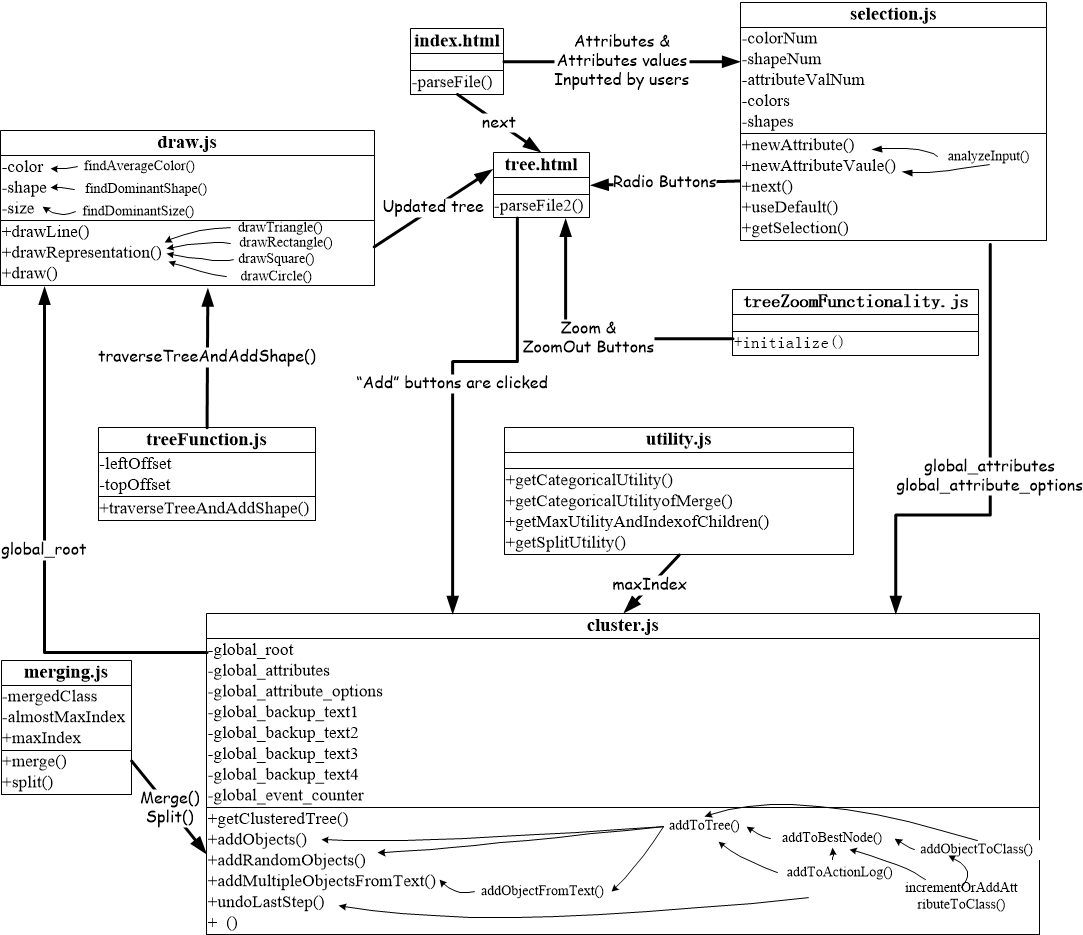
\includegraphics[width=400pt]{../images/class_diagram_for_Conceptual_Clustering.jpg}
    \caption{Class Diagram of TAILS Conceptual Clustering Module}
    \label{Fig:ClassDiagram}
\end{figure}

\subsection{The Sequence Diagram}
The sequence diagram is shown in Figure \ref{Fig:SequenceDigram}. It displays what actions from users can trigger which JavaScript file, the calling sequence of all the files and which function or variable is being transmitted between them.
\begin{figure}[h!]
    \centering
    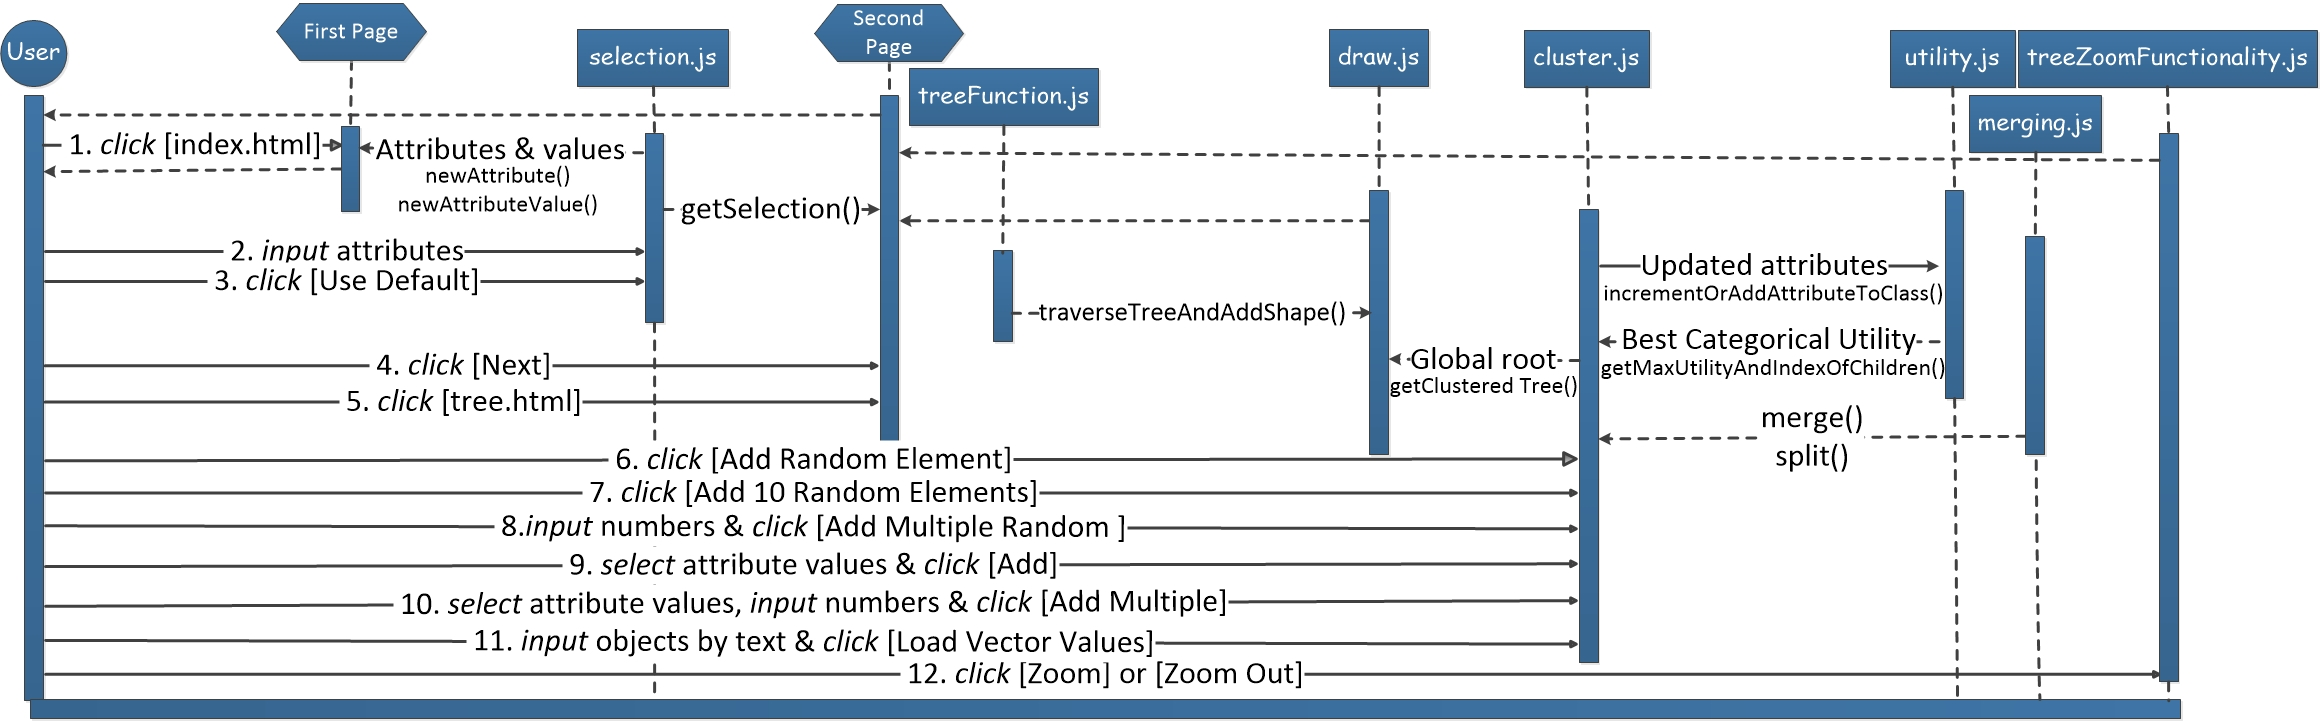
\includegraphics[width=400pt]{../images/sequence_diagram_for_Conceptual_clustering.jpg}
    \caption{Sequence Diagram of TAILS Conceptual Clustering Module}
    \label{Fig:SequenceDigram}
\end{figure}

\begin{comment}
\begin{itemize} \setlength{\itemsep}{0.01pt} %\itemsep-3pt
    \item Introduction,
    \item A user interface, and
    \item A classification tree visual.
\end{itemize}


\subsubsection{Introduction}
The introduction describes the use of the tool and explains the COBWEB algorithm. The description of the tool includes the instruction for custom input format and the procedures for inputting data. The explanation for the algorithm includes what specific operation is being carried out as a new object is added to the tree. The introduction not only shows how to use the simulation tool, but also relates the algorithm to the visual graphic tree generated by the algorithm, so that users can have a better understanding of how the COBWEB algorithm works.

\subsubsection{User Input}
Inputs for the conceptual clustering tool includes two parts: input for the attributes and attribute values and input for each object. There are three different ways for inputting attributes and values. System default supplies users with diverse attributes and various values. It's simple for users to get familiar with the COBWEB algorithm by the use of default attributes. Besides, the tool allows users to input their own data by the browser input or uploading a file. Either way, the attributes and values should be in the form of word only. No number or special characters are allowed. The other input is the object input by selecting specific attribute values defined by the first part. Adding one or multiple objects in fact generates a specific sequence for the input data. We have talked about the effect of the input orders for the tree generated in section 3.4. Users can also observe the effect by just playing the tool a little while.
\begin{itemize}\setlength{\itemsep}{0.01pt}
\item {Attributes and Attribute values}
\begin{itemize}\setlength{\itemsep}{0.01pt}
\item System default; 
\item Browser input;
\item And upload file of feature vectors.
\end{itemize}
\item {Input Sequence}
\end {itemize}
\subsubsection{Classification Tree Visual}
The classification tree will be generated while the object is being inputted. The user may either choose to add one object or multiple objects at a time.	The tool is able to generate tree for the selected objects or for random objects. For each node in the tree, there is a probabilistic concept label. Users can see the label by moving the mouse on the node. The label shows the conditional probability for each attribute value in the current cluster, which corresponds to $P(A_i=V_{ij}\left|C_k\right.)$, and the percentage of the current cluster against the whole tree which corresponds to $P(C_k)$.

\begin{figure}[h!]
    \centering
    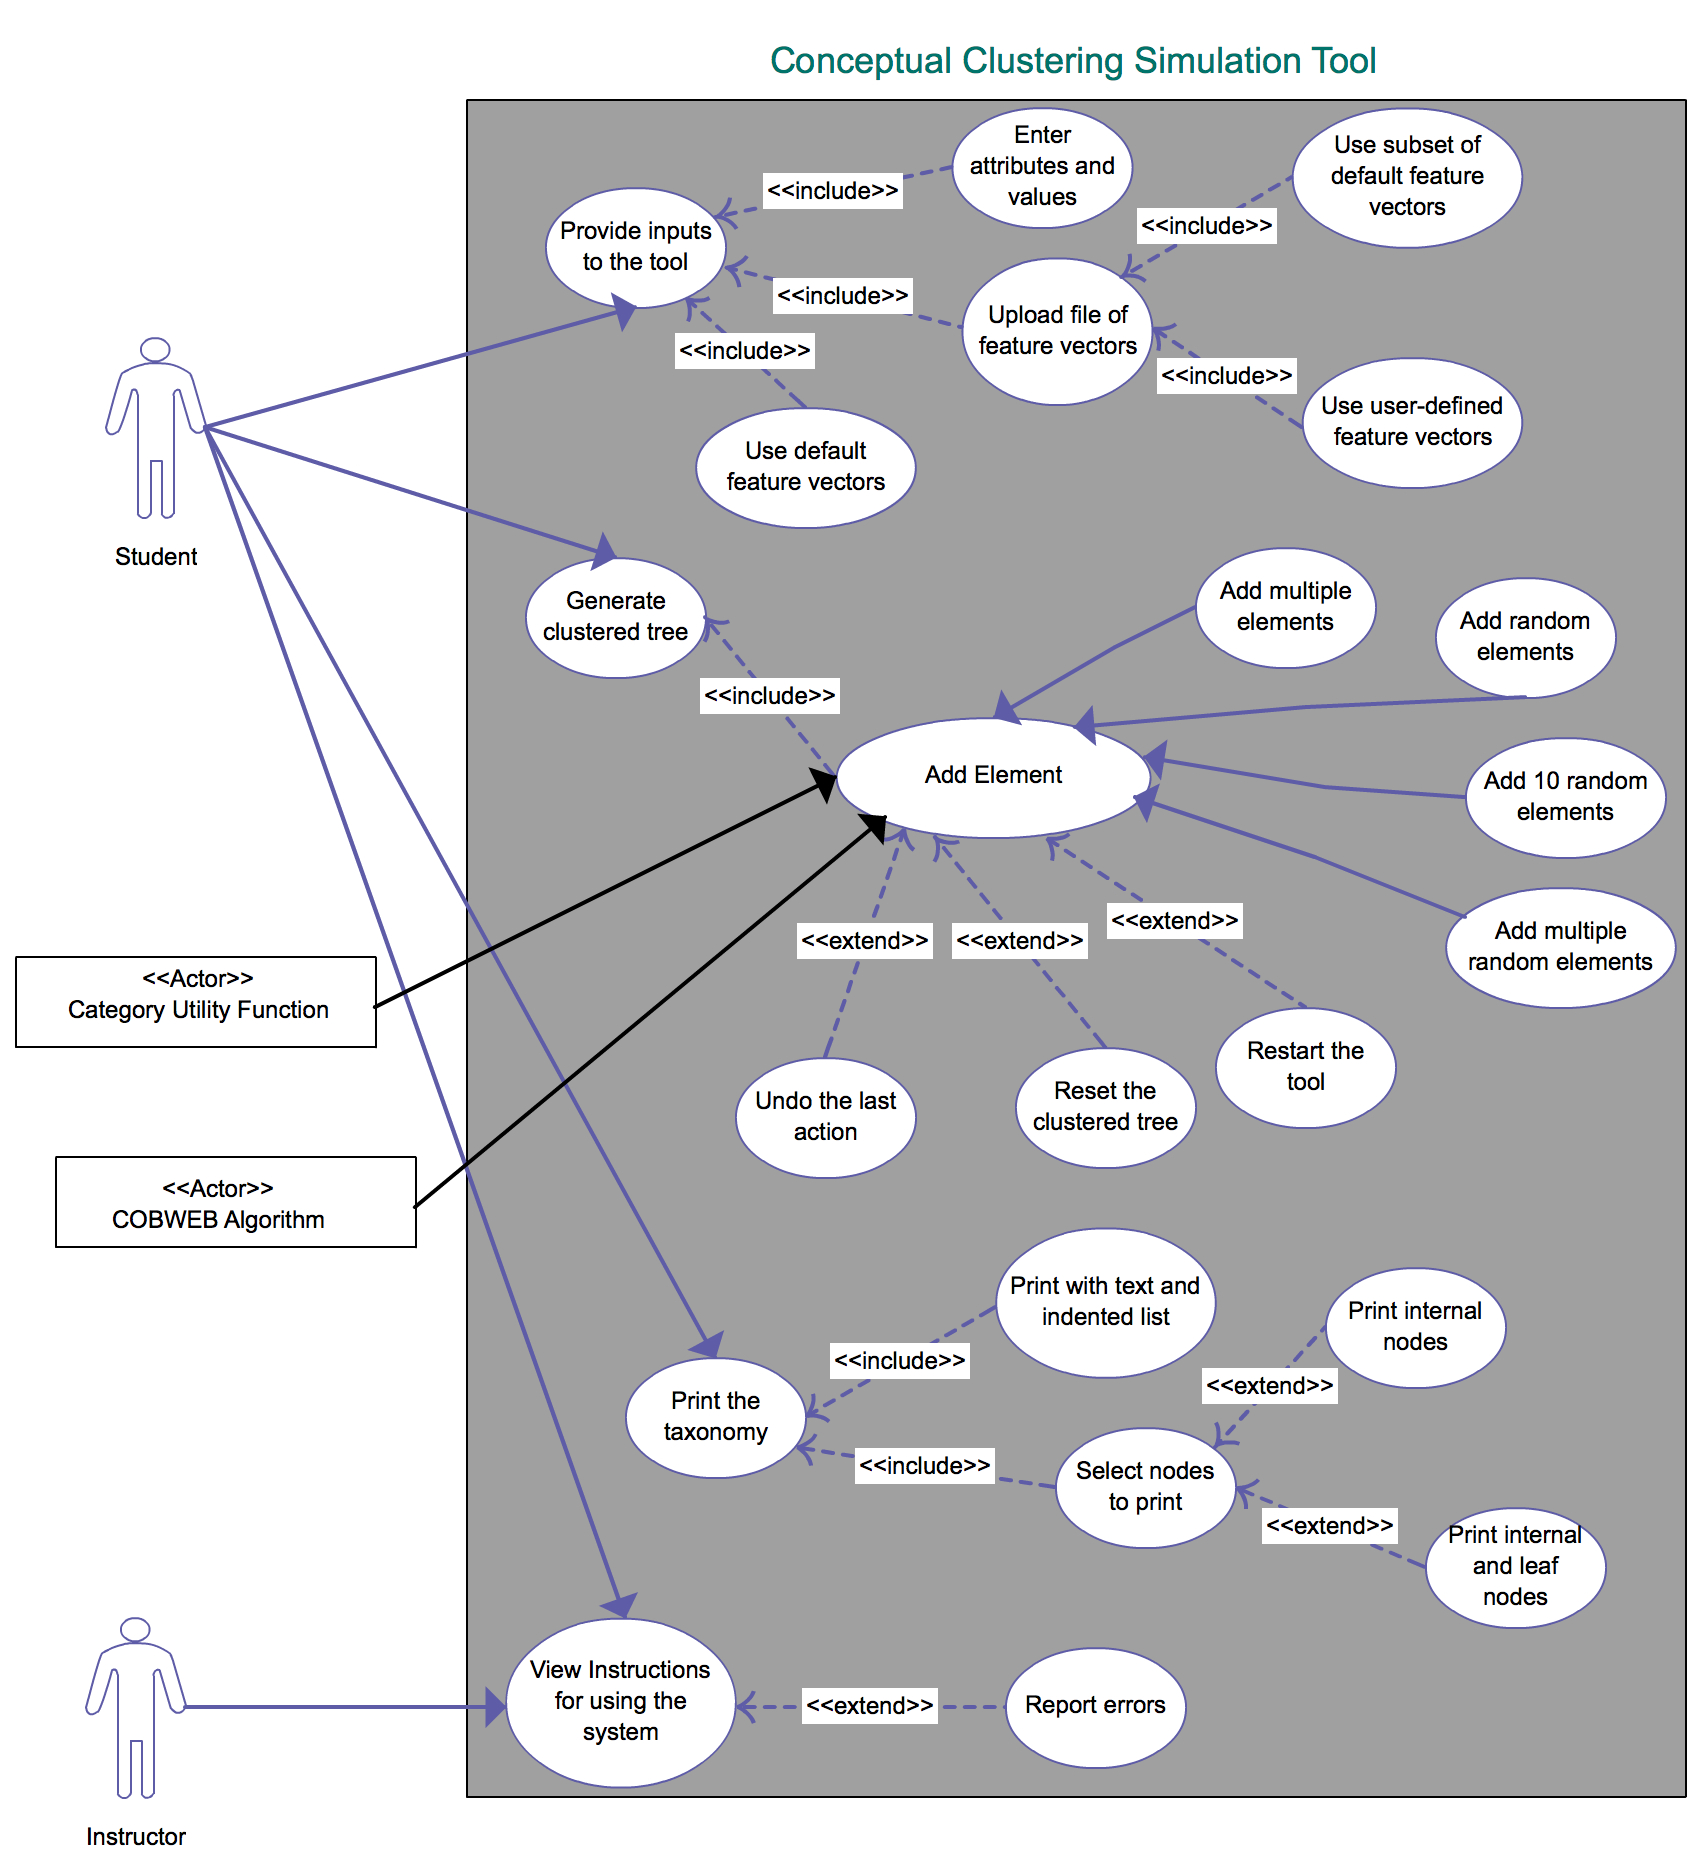
\includegraphics[width=400pt]{../images/Functional_CIM_Conceptual_Clustering.jpg}
    \caption{Use Case Diagram of TAILS Conceptual Clustering Module}
    \label{Fig:CIM}
\end{figure}

\end{comment}



% This module has the following requirements:

%\begin{enumerate}\itemsep-3pt
%\item There must be an introductory paragraph explaining what the module is and how to use it.
%\item The user must be able to select the start location.
%\item The user must be able to select the end location.
%\item The user must be able to select the search algorithm.
%\item The user must be able to run the program when they choose.
%\item The user must be able to see vertex names when the mouse hovers over any vertex.
%\item A graph visual portraying a search space must be created.
%\item A searchtree visual corresponding to the current actions of the search algorithm must be created.
%\end{enumerate}

%Requirement 1 requires a introductory text block on the webpage, requirements 2, 3, 4, and 5 correspond to user input which means the webpage
%must have a user interface component, requirement 6 will be a passive attribute of vertices, and requirements 7 and 8 will each be fulfilled by 
%providing the required visuals in subsections of the webpage.